\documentclass[12pt, 
hyperref={colorlinks=true, linkcolor=blue, urlcolor=cyan}]{beamer}
\usetheme{default} 

\setbeamertemplate{navigation symbols}{} %gets rid of navigation symbols
\setbeamertemplate{footline}{} %gets rid of bottom navigation bars
\setbeamertemplate{footline}[page number]{} %use this for page numbers

\setbeamertemplate{itemize items}[circle] %round bullet points
\setlength\parskip{10pt} % white space between paragraphs

\usepackage{wrapfig}
\usepackage{subfig}
\usepackage{setspace}
\usepackage{enumerate}
\usepackage{graphicx}
\usepackage{amsmath}
\usepackage{amsfonts}
\usepackage{amssymb}
\usepackage{amsthm}
\usepackage{tikz}
\usepackage[UKenglish]{isodate}
\usepackage{xcolor}
\cleanlookdateon

% the preamble
\title{BIOST 311: \\ Regression Methods for the Health Sciences}
\author{Kelsey Grinde and Brian Williamson}
\institute{UW Biostatistics}
\date{Spring 2018}

\begin{document}
% title slide
\begin{frame}
\titlepage\thispagestyle{empty}
\end{frame}

% make it 4.something
\setbeamertemplate{footline}{%
  \raisebox{5pt}{\makebox[\paperwidth]{\makebox[120pt]{\scriptsize Last updated \today}\hfill\makebox[10pt]{\scriptsize 4.\insertframenumber~~}}}}  \newcounter{chap1}{\value{1}}
\setcounter{framenumber}{\value{chap1}}

\begin{frame}
\frametitle{CHAPTER 4: SPECIAL TOPICS}
At the end of this chapter, the typical student should be able to:
\begin{itemize}
\item describe why you might not want to use a parametric model,
\item describe a nonparametric statistical model,
\item describe a statistical parameter, 
\item and other things related to Kelsey's work
\end{itemize}
\end{frame}

\begin{frame}
\frametitle{SECTION 1: {\small NONPARAMETRIC ESTIMATION AND INFERENCE}}
\framesubtitle{(by Brian Williamson)}

So far, in this course, you have explored how to answer scientific questions related to: \vspace{-0.3cm}
\begin{itemize}
\item causal associations,
\item associations (and prediction),
\item and effect modification,
\end{itemize} \vspace{-0.3cm}
using linear regression, logistic regression, or Cox proportional hazards regression.

You have also explored the necessary assumptions for these models to be valid.

Fundamentally, however, these tools \textcolor{red}{all make potentially restrictive assumptions} on the true data-generating mechanism (i.e., the process that truly creates the data as we see it).
\end{frame}

\begin{frame}
\frametitle{Common data analysis goals}
\begin{center}
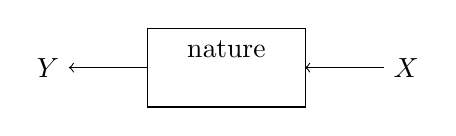
\begin{tikzpicture}
\node [left] at (0,1) {$Y$};
\node [right] at (4, 1) {$X$};
\draw [fill=white] (1,0.5) rectangle (3,1.5);
\node [above] at (2,1) {nature};
\draw [<-] (3,1) -- (4,1);
\draw [<-] (0,1) -- (1,1);
\end{tikzpicture}
\end{center}

Goals: \vspace{-0.3cm}
\begin{itemize}
\item \textcolor{blue}{\textit{Predict}} what the response will be with future predictors
\item Extract some information about the \textcolor{blue}{\textit{association}} between response and predictors in nature
\end{itemize} 
\end{frame}

% models, as you have seen them
\begin{frame}
\frametitle{Statistical models, as you have seen them}
Examples of statistical models: \vspace{6cm}
\end{frame}

\begin{frame}
\frametitle{Statistical models, as you have seen them}
Often, we use a \textcolor{red}{parametric model} for the relationship between our predictors and the response, for example: \vspace{-0.3cm}
\begin{itemize}
\item $Y \sim Bernoulli(p)$ 
\item $Y \sim N(0, 1)$
\item $E(Y \mid X) = \beta_0 + \beta_1 X$ 
\item $\text{logit} \{E(Y \mid X)\} = \beta_0 + \beta_1 X$
\end{itemize}

In the first two cases, \textcolor{magenta}{knowledge of a finite number of population parameters determines the entire distribution.}

In the second two cases, \textcolor{olive}{we specify (some function of) the conditional expectation as a linear function of a finite number of population parameters.}
\end{frame}

\begin{frame}
\frametitle{Statistical models, as you have seen them}
Advantages to a finite parametric model: \vspace{-0.3cm}
\begin{itemize}
\item \textcolor{blue}{simple} (too complex can be bad)
\item \textcolor{lime}{convenient} (we know how to fit them)
\end{itemize}

\end{frame}

\begin{frame}
\frametitle{Statistical models, as you have seen them}
Disadvantages to a finite parametric model: \vspace{-0.3cm}
\begin{itemize}
\item often, \textcolor{red}{the type of data at hand (rather than the scientific question) dictates the model used}, and parameters of interest are then determined by default:
\begin{itemize}
\item continuous outcome $+$ covariates $\rightarrow$ linear regression
\item binary outcome $+$ covariates $\rightarrow$ logistic regression
\item survival outcome $+$ covariates $\rightarrow$ proportional hazards regression
\end{itemize}
\item \textcolor{olive}{do we really care about these parameters?}
\item \textcolor{magenta}{what happens if the model is misspecified?}
\begin{itemize}
\item what are we estimating?
\item is inference valid for what we are actually estimating?
\end{itemize}
\end{itemize}
\end{frame}

% parameters, as you have seen them
\begin{frame}
\frametitle{Statistical parameters, as you have seen them}
Determine the statistical model (e.g., Bernoulli, linear model). 

\textcolor{magenta}{The parameters of interest define, or index, the model:} \vspace{-0.3cm}
\begin{itemize}
\item $p$ defines a $Bernoulli(p)$
\item $(\mu, \sigma)$ defines a $N(\mu, \sigma^2)$
\item $\beta_0, \beta_1$ define a simple regression model
\end{itemize}

\end{frame}

% breiman "modeling"
\begin{frame}
\frametitle{Common current approaches to modeling}
\begin{center}
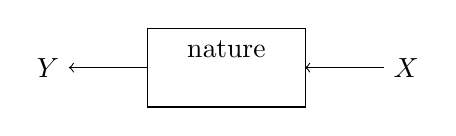
\begin{tikzpicture}
\node [left] at (0,1) {$Y$};
\node [right] at (4, 1) {$X$};
\draw [fill=white] (1,0.5) rectangle (3,1.5);
\node [above] at (2,1) {nature};
\draw [<-] (3,1) -- (4,1);
\draw [<-] (0,1) -- (1,1);
\end{tikzpicture}
\end{center}

Traditional statistical modeling:
\begin{center}
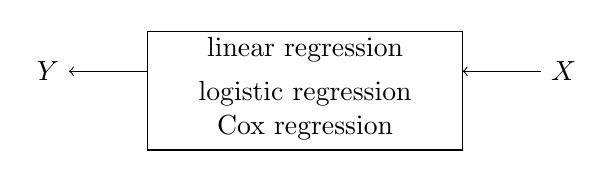
\begin{tikzpicture}
\node [left] at (0,1) {$Y$};
\node [right] at (6, 1) {$X$};
\draw [fill=white] (1,0) rectangle (5,1.5);
\node [above] at (3,1) {linear regression};
\node [below] at (3,1) {logistic regression};
\node [above] at (3,0) {Cox regression};
\draw [<-] (5,1) -- (6,1);
\draw [<-] (0,1) -- (1,1);
\end{tikzpicture}
\end{center}

Algorithmic modeling:

\begin{center}
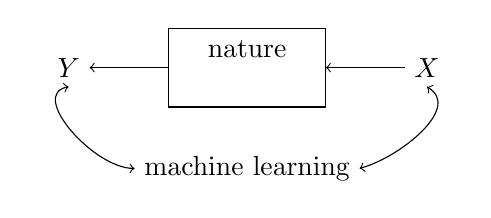
\begin{tikzpicture}
\node [left] (1) at (0,1) {$Y$};
\node [right] (2) at (4, 1) {$X$};
\draw [fill=white] (1,0.5) rectangle (3,1.5);
\node [above] at (2,1) {nature};
\draw [<-] (3,1) -- (4,1);
\draw [<-] (0,1) -- (1,1);
\node [below] (3) at (2,0) {machine learning};
\draw [<->] (2.south) to [out = -30, in = 15] (3.east);
\draw [<->] (1.south) to [out = 190, in = 180] (3.west);
\end{tikzpicture}
\end{center}
\end{frame}

% models, as I see them
\begin{frame}
\frametitle{Statistical models, as I see them}
Fundamentally, \textcolor{blue}{statistical models are collections of plausible probability distributions, and need not be indexed by a finite-dimensional parameter.}

We should \textcolor{blue}{put as much knowledge as possible into choosing this model}, \textcolor{green}{but make sure that the true data-generating mechanism will be contained in it.} This is where we ``model'' nature!
\begin{center}
\begin{tikzpicture}
\draw (0,0) ellipse (2.5cm and 2cm);
\node [below] at (1,-1) {$\mathcal{M}$}; 
\draw [fill] (-1, 1) circle [radius=0.05];
\node [right] at (-1,1) {$P_0$};
\end{tikzpicture}
\end{center}
\end{frame}

% parameters, as I see them
\begin{frame}
\frametitle{Statistical parameters, as I see them}
A \textbf{finite-dimensional parameter} takes as input a probability distribution, and outputs a real number (or a vector). \vspace{-0.3cm}
\begin{itemize}
\item[] e.g.: mean, variance, correlation, $\dots$
\end{itemize}

\begin{center}
\begin{tikzpicture}
\draw (0,0) ellipse (2.5cm and 2cm);
\node [below] at (1,-1) {$\mathcal{M}$}; 
\draw [fill] (-1, 1) circle [radius=0.05];
\node [right] at (-1,1) {$P_0$};
\draw [<->] (4, 0.5) -- (8, 0.5);
\draw[fill] (0,0) circle [radius=0.05];
\node [above] (0, 0) {$P$};
\draw [->] (0,0) to [out = -30, in = -90] (7, 0.5) node [above] {$\Psi(P)$};
\draw [fill] (7, 0.5) circle [radius = 0.05];
\node [below] at (4, -1.5) {$\Psi$};
\end{tikzpicture}
\end{center}

Our goal, typically, is to estimate the \textbf{true parameter value} $\psi_0 := \Psi(P_0)$ based on observations drawn from $P_0$.
\end{frame}

\begin{frame}
\frametitle{Statistical parameters, as I see them}
\begin{center}
\begin{tikzpicture}
\draw (0,0) ellipse (2.5cm and 2cm);
\node [below] at (1,-1) {$\mathcal{M}$}; 
\draw [fill] (-1, 1) circle [radius=0.05];
\node [right] at (-1,1) {$P_0$};
\draw [<->] (4, 0.5) -- (8, 0.5);
\draw[fill] (0,0) circle [radius=0.05];
\node [above] (0, 0) {$P$};
\draw [->] (0,0) to [out = -30, in = -90] (7, 0.5) node [above] {$\Psi(P)$};
\draw [fill] (7, 0.5) circle [radius = 0.05];
\node [below] at (4, -1.5) {$\Psi$};
\end{tikzpicture}
\end{center}

$\mathcal{M}$ \textcolor{green}{encodes our knowledge about nature.}

$P_0$ \textcolor{cyan}{is the true data-generating mechanism (unknown).}

$\Psi$ \textcolor{blue}{tells us about nature, and is something we can estimate.}
\end{frame}

% modeling culture
\begin{frame}
\frametitle{My modeling approach}
\textcolor{blue}{Writing the statistical model and parameter separately allow us to disentangle the parameter and estimation.}

Proposed workflow:
\begin{enumerate}
\item Define a statistical model (often nonparametric, or not indexed by a finite-dimensional parameter)
\item Define statistical parameter of interest
\item Choose an estimation procedure for this parameter
\end{enumerate}

However, steps 2 and 3 involve work: once a useful parameter is defined, it must be studied so that we can estimate it unbiasedly and obtain valid inference for it.
\end{frame}

% the model as a collection of probability distributions
%\begin{frame}
%\frametitle{Statistical models}
%Rather than restrict ourselves to a class of models that we can index by a finite parameter (e.g., regression coefficients), it is often useful to consider statistical models as more general objects.
%
%Statistical model: a group of probability distributions; should contain our true data-generating mechanism.
%
%\begin{tikzpicture}
%
%\end{tikzpicture}
%
%\end{frame}
%
%% the parameter as a map from the collection to the real line
%\begin{frame}
%\frametitle{Statistical parameters: more than just $\beta$s?}
%Just like the parameters in our linear model, statistical parameters are functions of the true data-generating mechanism.
%
%However, now a statistical parameter is a function that takes as input a probability distribution, and outputs a real number.
%
%We can now define parameters of arbitrary distributions, without making any assumptions on the model!
%
%For example, the mean as a statistical parameter: $\mu(P) = \int x dP(x)$; or the conditional mean as a statistical parameter: $\mu_X(P) = E(Y \mid X) = \int y dP(Y \mid X)$.
%\end{frame}
%
%% procedure that separates statistical model and parameter from estimation
%\begin{frame}
%\frametitle{New paradigm for estimation}
%Defining a statistical parameter as a function of the statistical model, rather than the estimation procedure (e.g., linear regression), means that we can disassociate the two processes:
%\begin{enumerate}
%\item Define my statistical parameter
%\item Estimate the relevant components using potentially complex methods
%\item Plug these estimates into the form for the parameter
%\item Correct the resulting estimate for the fact that flexible techniques were used
%\end{enumerate}
%
%Fundamentally: \textcolor{blue}{the statistical parameter of interest doesn't have to be tied to your estimation technique.}
%\end{frame}


% introduce the variable importance problem, in the context of HIV vaccine
\begin{frame}
\frametitle{Case study: variable importance}
A new frontier in HIV-1 vaccine research studies \textcolor{blue}{broadly neutralizing antibodies}: HIV-1 is diverse and mutates quickly, so successful antibodies against HIV-1 must be able to recognize and neutralize many strains.

VRC01: \vspace{-0.3cm}
\begin{itemize}
\item a broadly neutralizing antibody against HIV-1
\item isolated from a donor chronically infected with HIV-1 for 15 years
\item neutralizes over 80\% of $> 600$ viral strains tested
\end{itemize}

The Antibody Mediated Prevention (AMP) trials, expected to finish in 2020, \textcolor{blue}{assess the efficacy of VRC01 in preventing HIV-1 infection}.
\end{frame}

% variable importance
\begin{frame}
\frametitle{Case study: variable importance}
Part of the pre-planned analysis of these data involves testing those viruses that do cause infection, even in the presence of VRC01.

\textcolor{blue}{Differences in prevention efficacy based on features of these viruses give us information about how VRC01 works to prevent infection}, and give us \textcolor{green}{clues about how to develop an effective vaccine.}

I am primarily interested in features of the HIV-1 genotype, but there are \textcolor{red}{many ways} to define an HIV-1 genotype; this implies that \textcolor{red}{if we test each amino acid feature, and apply a multiple comparisons correction, it will be difficult to detect effects. }
\end{frame}

% variable importance!
\begin{frame}
\frametitle{Case study: variable importance}
Fortunately, there are publicly available data on the neutralization sensitivity of HIV-1 viruses to VRC01. I am currently collaborating with researchers at the Fred Hutchinson Cancer Research Center to:
\begin{itemize}
\item develop an algorithm that has \textcolor{green}{good accuracy in predicting neutralization sensitivity} from HIV-1 amino acid features, and
\item \textcolor{blue}{rank amino acid features by their importance in predicting neutralization sensitivity}, and advance the top ranked features to the AMP analysis
\end{itemize}

Fitting \textcolor{green}{complex machine learning-based methods} achieves the first objective; the second objective is a \textcolor{blue}{bit more nuanced}.
\end{frame}

% how would we address this using linear regression?
\begin{frame}
\frametitle{Case study: variable importance}
Variable importance in linear regression: e.g., $E(Y \mid X_1, X_2) = \beta_0 + \beta_1 X_1 + \beta_2 X_2$
\begin{itemize}
\item $\beta_1$: difference in mean $Y$ for two groups differing by one unit in $X_1$, with the same value of $X_2$
\item $X_1$ has no effect on $Y$ if $\beta_1 = 0$ (i.e., is unimportant)
\item estimate importance (i.e., deviation from the null) with $\lvert (\hat{\beta}_1 - 0)/SE(\hat{\beta}_1) \rvert$
\end{itemize}

However, it is possible that our variables of interest are important in other ways besides the linear association. If the linear model doesn't hold, \textcolor{red}{then these variable importance estimates are meaningless.}
\end{frame}


% variable importance parameter
\begin{frame}
\frametitle{Case study: variable importance}
In this context, we define variable importance using a nonparametric extension of $R^2$ or ANOVA-derived variable importance:
\begin{align*}
\Psi_s(P) = &\ \frac{\int \{E_P(Y \mid X) - E_P(Y \mid X_{(-s)})\}^2 dP(x)}{var_P(Y)}
\end{align*}

\textcolor{cyan}{This measures the additional proportion of the variability in the outcome explained by including the features $X_s$ in the regression} ($s$ can index a single feature or group of features).

\textcolor{red}{Coming up with a parameter can be hard work:} this particular parameter resulted from multiple consultations between statisticians and epidemiologists.

However, this work is worth it: at the end of the day, you are estimating something you care about!
\end{frame}

% how to estimate it?
\begin{frame}
\frametitle{Case study: variable importance}
\vspace{-0.75cm}
\begin{align*}
\Psi_s(P) = &\ \frac{\int \{E_P(Y \mid X) - E_P(Y \mid X_{(-s)})\}^2 dP(x)}{var_P(Y)}
\end{align*}
\vspace{-0.4cm}
I need to estimate four objects:
\begin{itemize}
\item the probability distribution of the $X$ data
\item the conditional expectation given $X$
\item the conditional expectation given $X_{(-s)}$
\item the variance of $Y$
\end{itemize}

\textcolor{blue}{The first and last components are easy}: take the empirical variance, and take a simple average once I have the middle two components.

\textcolor{red}{The middle two components are where I can run into trouble if I make incorrect assumptions. }
\end{frame}

% ML tools
\begin{frame}
\frametitle{Estimating a conditional mean}
So far, this quarter, we have studied three methods for estimating conditional means (also called \textcolor{blue}{regression functions}):
\begin{itemize}
\item linear regression,
\item logistic regression, and
\item Cox proportional hazards regression.
\end{itemize}

Each of these tools makes the fundamental assumption that some function of the conditional mean is linear in the model parameters, which is potentially quite restrictive.

More model-agnostic regression techniques are known colloquially as ``machine learning'' tools.
\end{frame}

% the bias-variance tradeoff
\begin{frame}
\frametitle{Estimating a conditional mean}
Typically, machine learning-based methods involve 

\end{frame}

% why that's a problem for us

% how we get around it

% simulation results showing how bad it can be not to account for it

% results from the VRC01 study

% conclude


\end{document}
